% FistBump research poster
% Built on the Gemini beamerposter theme (https://github.com/anishathalye/gemini, MIT License; see LICENSE.md)

\documentclass[final]{beamer}

% ====================
% Packages
% ====================

\usepackage[T1]{fontenc}
\usepackage{lmodern}
\usepackage[size=a1,scale=1.35]{beamerposter}
\usetheme{gemini}
\usecolortheme{nott}
\usepackage{graphicx}
\usepackage{booktabs}
\usepackage{tikz}
\usetikzlibrary{arrows.meta,positioning}
\usepackage{anyfontsize}

% ====================
% Lengths
% ====================

% Three columns: (N+1)*\sepwidth + N*\colwidth = \paperwidth
\newlength{\sepwidth}
\newlength{\colwidth}
\setlength{\sepwidth}{0.025\paperwidth}
\setlength{\colwidth}{0.3\paperwidth}

\newcommand{\separatorcolumn}{\begin{column}{\sepwidth}\end{column}}

% ====================
% Title
% ====================

\title{FistBump: A Local-First Job Application Assistant}

\author{Tyler McGuire \and Joe Cooney \and Tyler Goodman \and Aron Magnusson}

\institute[shortinst]{College of Charleston, Department of Computer Science}

% ====================
% Footer
% ====================

\footercontent{
  \href{https://github.com/tlmcguire/fistbump}{github.com/tlmcguire/fistbump} \hfill
  v0.4.0, November 25, 2026 \hfill
  Tauri v2 + Go + SQLite}

% ====================
% Logos
% ====================

\logoright{
\includegraphics[height=6cm]{logos/pico.png}}

% ====================
% Body
% ====================

\begin{document}

% College of Charleston logo, top left
\addtobeamertemplate{headline}{}
{
    \begin{tikzpicture}[remember picture,overlay]
      \node [anchor=north west, inner sep=3cm] at ([xshift=-2.5cm,yshift=0.5cm]current page.north west)
      {
\includegraphics[height=4.5cm]{logos/cofc.eps}};
    \end{tikzpicture}
}

\begin{frame}[t]
\begin{columns}[t]
\separatorcolumn

% ====================
% Column 1: problem, requirements, design rule
% ====================

\begin{column}{\colwidth}

  \begin{block}{The problem}

    Every posting asks for a slightly different set of skills, and tailoring a
    resume for each one takes hours. Automated rewriters can invent claims the
    applicant never made, while job listings are fragmented across multiple
    ATS platforms. FistBump keeps search, the master resume, saved jobs,
    drafts, and application tracking on the user's machine—and nothing changes
    in the resume until the user approves it.

  \end{block}

  \begin{block}{Requirements and current status}

    \begin{tabular*}{\linewidth}{@{\extracolsep{\fill}} l c l}
      \toprule
      \textbf{Requirement} & \textbf{Phase} & \textbf{Status} \\
      \midrule
      FR-1 Master resume \& custom sections & 3+ & Met \\
      FR-2 Skill gaps, pay \& COL analysis & 1, 4 & Met \\
      FR-3 Accept, reject or edit revisions & 5, 8 & Met \\
      FR-4 Export PDF (5 styles), DOCX, MD & 6+ & Met \\
      FR-5 Jobs, tracker, drafts \& backup & 3--7+ & Met \\
      FR-6 Windows, macOS, Linux installers & 9 & Met \\
      FR-7 Open Greenhouse, Lever, Ashby & 1+ & Met \\
      FR-8 Search 1,300+ boards (46 fields) & 2+ & Met \\
      FR-9 Import PDF, DOCX, ODT, TXT, MD & 3+ & Met \\
      NFR-5 Install under 250 MB & 9+ & Met (Tauri v2) \\
      \bottomrule
    \end{tabular*}

    \vspace{0.5em}

    Migrating the desktop host from Electron (395 MB on Apple silicon) to
    Tauri v2's native system webview and on-demand \texttt{llama-server}
    downloads brought the installer well below the 250 MB target.

  \end{block}

  \begin{alertblock}{Design rule}

    Every AI change is a reviewable suggestion: accept, reject, or edit with
    visible word-level diffs before export. Skill-gap and cost-of-living
    analyses are deterministic (no LLM) and finish in under 1.5 s. For
    missing skills, the Honest Keyword Bridge offers visible framing
    (``Currently learning X'') with zero hidden text.

  \end{alertblock}

  \begin{block}{References}

    \nocite{*}
    \tiny{\bibliographystyle{plain}\bibliography{poster}}

  \end{block}

\end{column}

\separatorcolumn

% ====================
% Column 2: architecture and the app
% ====================

\begin{column}{\colwidth}

  \begin{block}{Architecture}

    \begin{center}
    \begin{tikzpicture}[
        box/.style={draw, rounded corners, align=center, font=\small,
                    minimum width=0.85\colwidth, minimum height=0.9cm,
                    inner sep=5pt},
        flow/.style={-{Stealth[length=2.5mm]}, thick}]
      \node[box, fill=gray!10] (ui) {Renderer: vanilla JS/CSS views\\
        Home, Tracker, Jobs (Find/Paste/Saved), Resume, Tailor, Settings};
      \node[box, fill=gray!10, below=0.28cm of ui] (pre) {Bridge: \texttt{tauri-bridge.js} (\texttt{window.api})\\
        typed IPC channel dispatch};
      \node[box, fill=gray!10, below=0.28cm of pre] (main) {Tauri v2 Rust host (\texttt{src-tauri})\\
        native dialogs, updater, sidecar lifecycle, per-launch token};
      \node[box, fill=gray!10, below=0.28cm of main] (go) {Go backend \texttt{fistbump-core}\\
        local HTTP API, ATS search, PDF/DOCX/ODT parser, local/remote AI};
      \node[box, fill=gray!10, below=0.28cm of go] (db) {SQLite on disk + local JSON backup/restore};

      \draw[flow] (ui) -- (pre);
      \draw[flow] (pre) -- (main);
      \draw[flow] (main) -- (go);
      \draw[flow] (go) -- (db);
    \end{tikzpicture}
    \end{center}

    The webview has no direct filesystem or shell access, and every local HTTP
    call carries a per-launch bearer token. Outbound traffic contacts public
    ATS boards only on user search/open, and a remote AI provider only if
    configured.

  \end{block}

  \begin{block}{The app}

    \begin{center}
    \begin{tabular}{cc}
      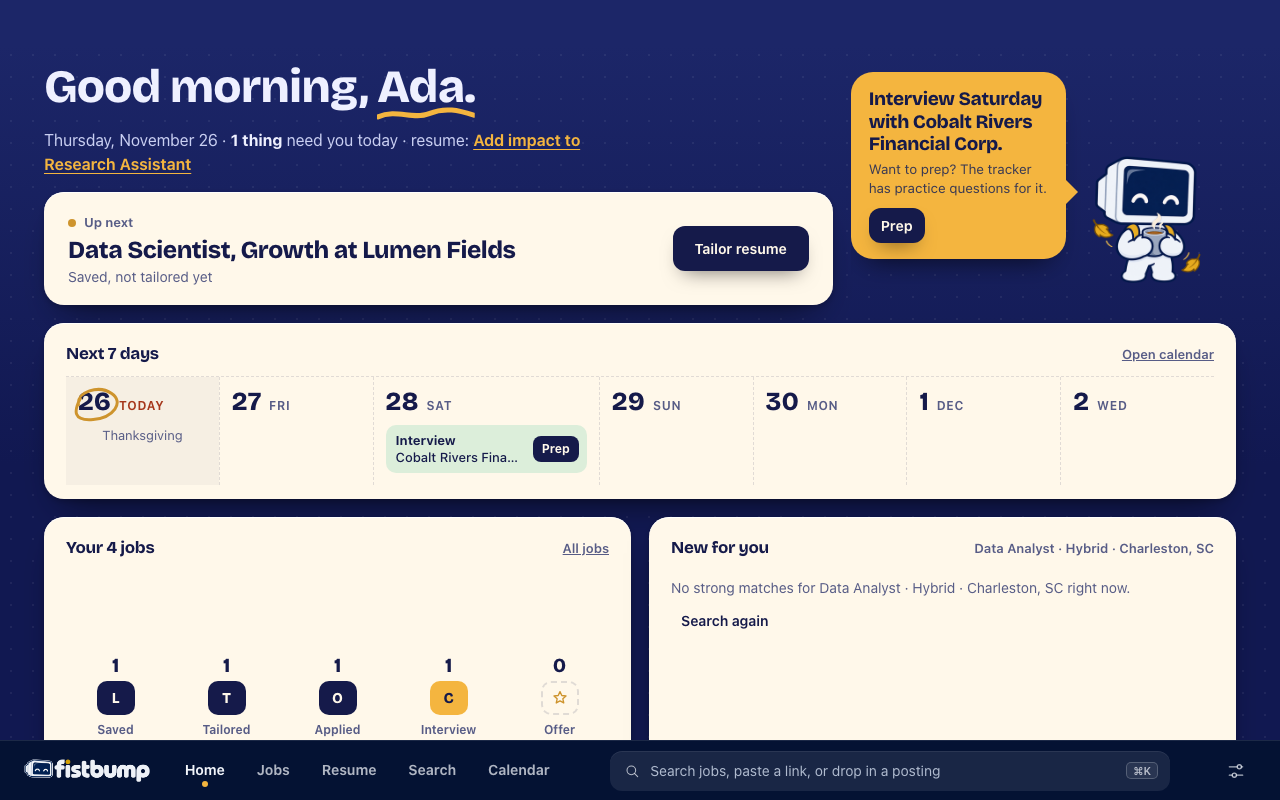
\includegraphics[width=0.41\colwidth]{../images/home.png} &
      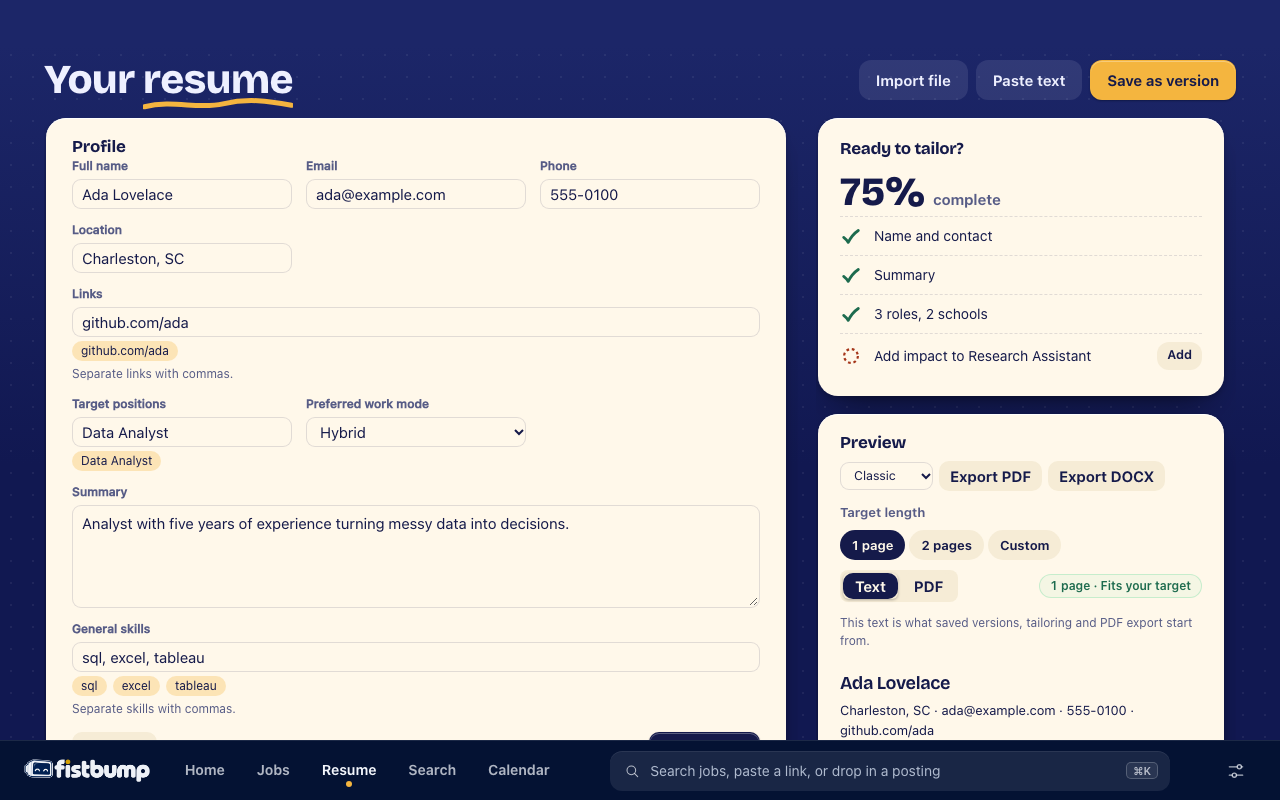
\includegraphics[width=0.41\colwidth]{../images/resume.png} \\
      {\footnotesize Home: follow-ups and jobs to tailor} &
      {\footnotesize Master resume: 5-style PDF \& DOCX} \\[0.45em]
      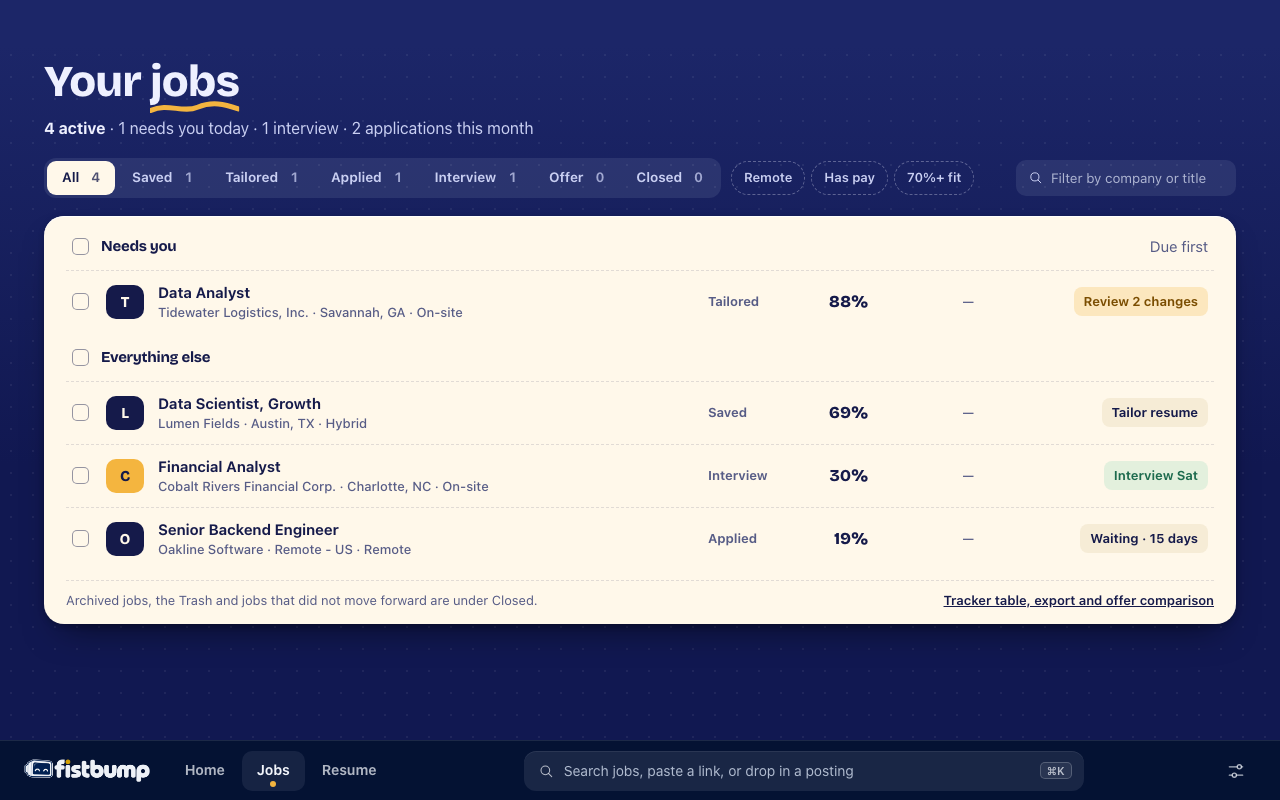
\includegraphics[width=0.41\colwidth]{../images/jobs.png} &
      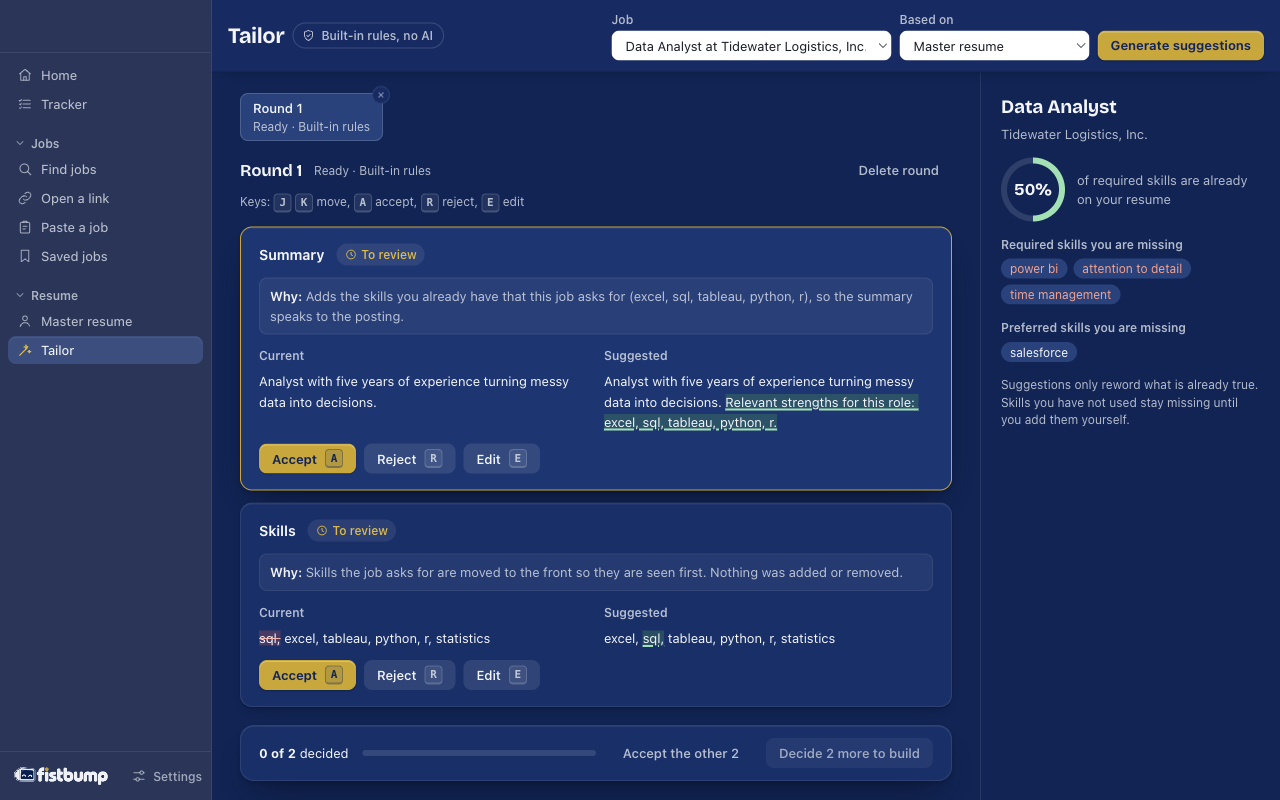
\includegraphics[width=0.41\colwidth]{../images/tailor.png} \\
      {\footnotesize Job detail: ATS source, fit \& COL} &
      {\footnotesize Tailor: diffs, keyword bridge \& drafts} \\[0.45em]
      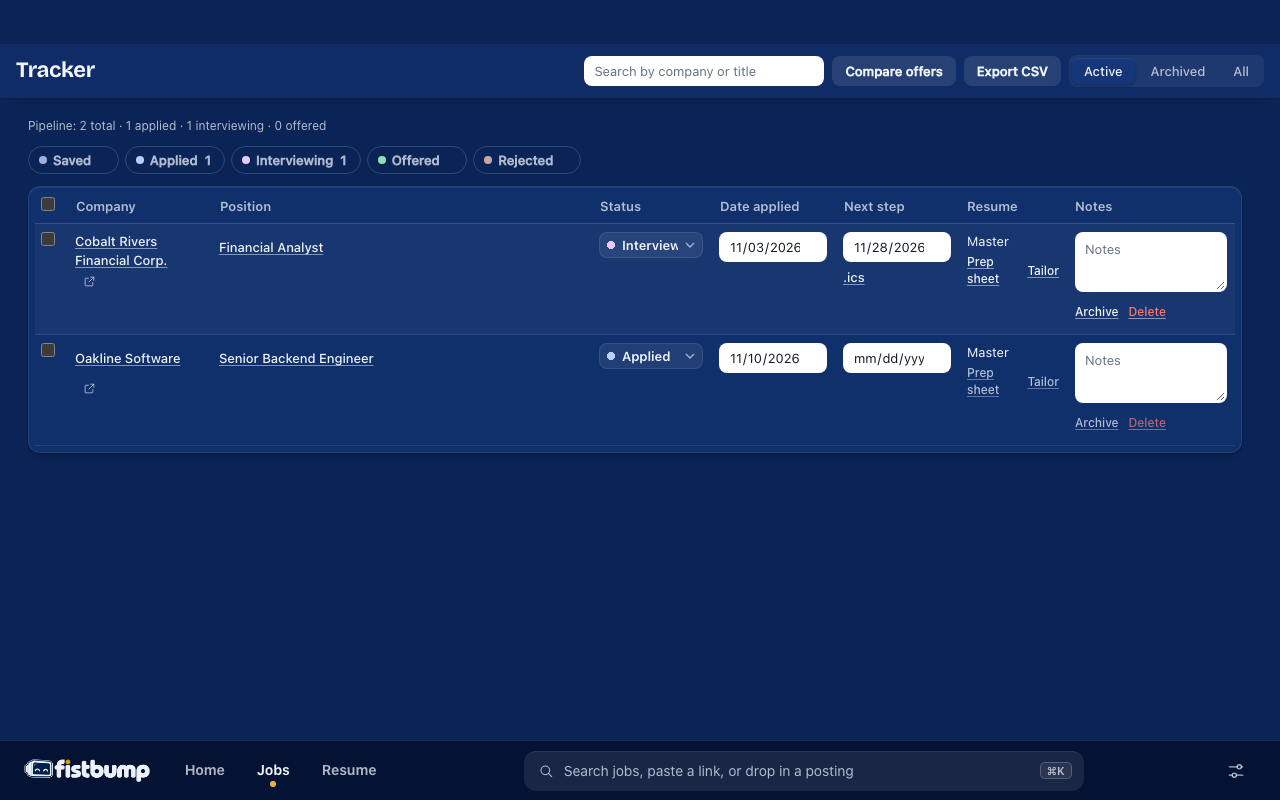
\includegraphics[width=0.41\colwidth]{../images/tracker.png} &
      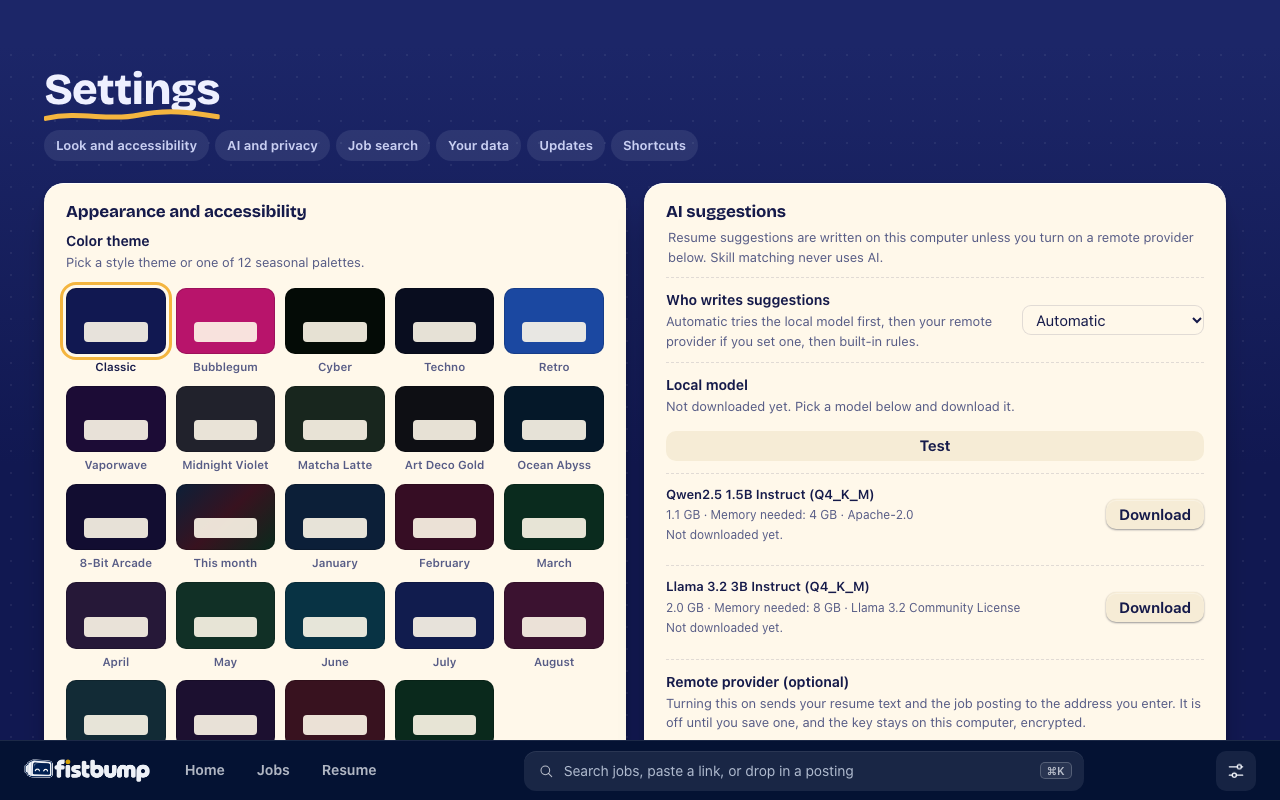
\includegraphics[width=0.41\colwidth]{../images/settings.png} \\
      {\footnotesize Tracker: prep sheets \& offer compare} &
      {\footnotesize Settings: AI, watchlists \& backup} \\
    \end{tabular}
    \end{center}

  \end{block}

\end{column}

\separatorcolumn

% ====================
% Column 3: timeline, what shipped, limits, code & team
% ====================

\begin{column}{\colwidth}

  \begin{block}{Project milestones}

    \begin{tabular*}{\linewidth}{@{\extracolsep{\fill}} c l l}
      \toprule
      \textbf{Phase} & \textbf{Delivers} & \textbf{Status} \\
      \midrule
      1--2 & Multi-ATS search, links, saved searches & Done \\
      3--4 & Resume builder, PDF/DOCX/ODT/MD import & Done \\
      5--6 & Tailoring loop, 5 PDF styles, DOCX export & Done \\
      7 & Tracker, prep sheets, offer comparison & Done \\
      8 & Local (\texttt{llama-server}) \& remote AI, drafts & Done \\
      9 & Tauri v2 migration, CI \& installers & Released \\
      \bottomrule
    \end{tabular*}

  \end{block}

  \begin{block}{What is shipped in v0.4.0}

    \begin{itemize}
      \item \textbf{Multi-ATS search:} 1,300+ Greenhouse, Lever, and Ashby boards across 46 industries, custom watchlists, ATS filters, saved searches with ``New'' badges, and cited pay/COL ratings.
      \item \textbf{Resume \& exports:} Import PDF, DOCX, ODT, TXT, or MD (with hidden-text stripping); custom sections \& ordering; 1-page fit audit; 5 PDF styles and DOCX export.
      \item \textbf{Tailor \& drafts:} Word-level diffs, Honest Keyword Bridge, cover letter \& Q\&A drafts, and dismissible job suggestions.
      \item \textbf{Tracker \& data:} Bulk delete/status, pipeline \& skill-gap stats, printable interview prep sheets, side-by-side offer comparison, CSV/\texttt{.ics} export, and JSON backup/restore.
    \end{itemize}

  \end{block}

  \begin{alertblock}{Known limits}

    \begin{itemize}
      \item Cross-platform installers (Windows, macOS, Linux) are currently unsigned.
      \item ATS platforms beyond Greenhouse, Lever, and Ashby remain paste-only.
      \item Skill matching uses a curated technical dictionary strongest for software and data roles.
      \item The local SQLite database is not encrypted at rest (API keys are encrypted).
    \end{itemize}

  \end{alertblock}

  \begin{block}{Code and team}

    Source and releases: \href{https://github.com/tlmcguire/fistbump}{github.com/tlmcguire/fistbump}.
    Automated test suite: 462 Go tests, 34 frontend JS tests, and 9 Rust host tests
    (505 total) running in CI across Ubuntu, macOS, and Windows.
    Team: Tyler McGuire, Joe Cooney, Tyler Goodman, and Aron Magnusson.

  \end{block}

\end{column}

\separatorcolumn
\end{columns}
\end{frame}

\end{document}
